\section[Broken symmetries]{Broken continuous symmetries and Goldstone-modes}

Both of the previous examples, the BCS- and Hubbard-model, have shown that a system where the Hamiltonian is invariant under a continuous symmetry group ($U(1)$ in both cases), the ground state, which the system chooses, doesn't need to respect the symmetry. This are examples of broken symmetries, and because the system ``breakes it on its own'', we say that the systems have spontaneously broken (continuous) symmetries. In the following, we will examine an important consequence of these broken symmetries. Note that this does not apply to discrete symmetries, like e.g. Ising-model.  

BCS-model: 

\begin{equation*}
    f^{\text{MF}}(\ad, a) = f(\abs{a}^2) \quad \expval{\ad} \neq 0 \neq \expval{a}.
\end{equation*}

$U = \infty$ Hubbard model: 

\begin{equation*}
    f^{\text{MF}}(\bd, d) = f(\abs{b}^2) 
\end{equation*}

\begin{equation*}
    \abs{\Delta} = \abs{a}, \abs{b}. 
\end{equation*}

In \cref{fig:free_broken1} we see that there is two global minima of $f^{\text{MF}}$ for non-zero $\Delta$'s. These are both stable. 
\begin{figure}
	\centering
	\begin{subfigure}{0.4\textwidth}    
		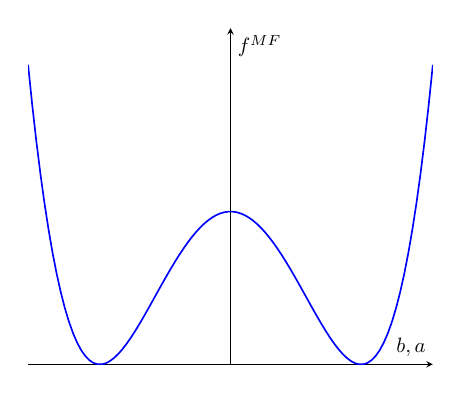
\begin{tikzpicture}[scale=0.75]
	\begin{axis}[
	ticks = none,
	xlabel = {$b,a$},
	ylabel = $f^{\text{MF}}$,
	x label style={at={(axis description cs:1,0.1)}, anchor = west},
	y label style={at={(axis description cs:0.15,1)},rotate=-90,anchor=south},
	ymax = 2,	
	axis lines = middle]
	
	
	
	\addplot[thick,
	domain=-2:2, 
	samples=100, 
	color=blue]{- x^2 + 0.3*x^4 + 1};
	
	\end{axis}
      %\draw[->] (-4,0) -- (4,0) node[right] {$b, a$};
      %\draw[->] (0,-4) -- (0,4) node[above] {$f^{MF}$};
      %\draw[blue] plot[samples=200,domain=-2:2] function {};
\end{tikzpicture}
		\caption{$|\Delta| \ne 0$}
		\label{fig:free_broken1}
	\end{subfigure}
	\hfill
	\begin{subfigure}{0.4\textwidth}
		\begin{tikzpicture}[scale = 0.75]
	\begin{axis}[
	ticks = none,
	xlabel = {$b,a$},
	ylabel = $f^{\text{MF}}$,
	x label style={at={(axis description cs:2,0.1)}, anchor = west},
	y label style={at={(axis description cs:0.15,2)},rotate=-90,anchor=south},
	ymax = 4,	
	axis lines = middle]
	
	
	
	\addplot[thick,
	domain=-2:2, 
	samples=100, 
	color=blue]{0.7*x^2 + 0.5};
	
	\end{axis}



      %\draw[->] (-4,0) -- (4,0) node[right] {$b, a$};
      %\draw[->] (0,-4) -- (0,4) node[above] {$f^{MF}$};
      %\draw[blue] plot[samples=200,domain=-2:2] function {};
\end{tikzpicture}
		\caption{$|\Delta| = 0$}
		\label{fig:free_broken_2}	
	\end{subfigure}
	\label{fig:free_broken}
\end{figure}

\begin{equation*}
    \pdv{f^{\text{MF}}(\Delta^2)}{\Delta} = 2\Delta f^{'}(\Delta^2) 
\end{equation*}

\begin{equation*}
     \abs{\Delta} = 0
\end{equation*}

In \cref{fig:free_broken_2} we see that $f^{\text{MF}}$ has one global minima at $\Delta = 0$. This minima is also stable. 

We have seen that generally $\expval{a}$ and $\expval{b}$ are complex order parameters. We can therefore treat $f^{\text{MF}}$ as a function of a complex variable, while it is independent of the phase of the complex number. In the case of $\abs{\Delta} = 0$, the phase is ill-defined at $f^{\text{MF}}_{min}$. In the case of $\abs{\Delta} \neq 0$, the situation is a little bit different. Then we can rotate the corresponding graph around the y-axis ($f^{\text{MF}}$), and we obtain the following kind of graph

% \begin{figure}
%     \centering
% \begin{tikzpicture}[scale =1.5]
%     \begin{axis}[
%         hide axis,
%         samples=50,
%         domain=0:360,
%         y domain=0:1.25
%         ]
%     \addplot3 [surf, shader=flat, draw=blue!70!white, fill=white, z buffer=sort] ({sin(x)*y}, {cos(x)*y}, {(y^2-1)^2});
%     \end{axis}
% \end{tikzpicture}
%     
% \end{figure}


We see that the minima of the free energy is infinetly degenerate, because it is independent of the phase $\varphi$: 

\begin{align*}
    f^{\text{MF}}(\Delta, \Delta^*) = f^{\text{MF}}(\abs{\Delta}, \varphi) = f^{\text{MF}}(\abs{\Delta}) \\
    \Delta = \abs{\Delta}\e^{i\varphi}. 
\end{align*}

This means that phase fluctuations cost no energy, but fluctuations in the radial $\abs{\Delta}$ direction does.
\begin{itemize}
	\item $\abs{\Delta}$-amplitude fluctuations: Longitudinal fluctuations.
	\item $\varphi$-fluctuations: Transverse fluctuations. 
\end{itemize}

We say that the longitudinal fluctuations are "massive" and the traversal fluctuations are "massless". The massless fluctuations correspond to Goldstone-modes, which has a finite interaction range. We have seen that a broken symmetry ($\Delta \neq 0$) means that there exist Goldstone-modes. 

In our case, the order parameter where comples, which means that it has two real components. Here we got one infinite degeneracy in the phase, which corresponded to one Goldstone mode. Generally in our study, if $\Delta$ has n components, we get $n-1$ Golstone-modes.  

The existence of the Goldstone-modes makes it apparently problematic to define a fluctuation-calculation around the stationary point, since the Goldstone-modes corresponds to (at least one) zero eigenvalue of the fluctuation propagators. 
\begin{align*}
    S = S^{\text{MF}} + \Tr \ln D^{-1} \\ 
    Z = \e^{S^{\text{MF}}}\frac{1}{\det D^{-1}} \\ 
    D^{-1} = \prod_i \lambda_i \quad \quad \exists j : \lambda_j = 0 
\end{align*}

In order to investigate small fluctuations around a mean-field theory, it is of course intolerable to have this problem. It turns out that this is an apparent problem which we can avoid, as we will see. 

We will look at Gaussian fluctuations around a spontaneously broken continuous symmetry. The following effective action isn't approximated, but we will for the sake of the argument and simplicity look at a real field with real rotational invariance (e.g. XY-model, where the spins can point in any direction in the plane). I emphasise however that the discussion is general. 

\begin{align*}
    Z = \int \D \p \e^{S[\p]} \\ 
    \fdv{S}{\p} = 0 \quad \quad  \p = \p_0
\end{align*}

where $\p$ is a function of $x = (\Vec{x_0}, \tau)$. $\p_0$ contains a parameter $\theta$ which describe the symmetry-transformation of the symmetry that is spontaneously broken. It can e.g. be the parameter describing the ground state degeneracy ("circular minimum") in the rotated graph of $f^{\text{MF}}$ above. We expand to gaussian order in $S$:

\begin{align*}
    Z = \e^{S^{\text{MF}}}\int \D \p \e^{-\frac{1}{2}\sum_{x,y} (\p(x) - \p_0(x)) A (\p(y) - \p_0(y))} \\
    A = \fdv{^2S}{\p_0(x) \delta \p_0(y)}
\end{align*}

Naively, this will be something like 

\begin{align*}
    Z = \e^{S^{\text{MF}}} \frac{1}{\sqrt{\det A}}
\end{align*}

but because of the Goldstone-modes, there is an apparent divergence in the fluctuations due to the zero eigenvalue. It seems like any attempt at doing mean-field theory when the symmetry is broken is doomed to fail. Nevertheless, we know that e.g. the mean-field theory of BCS-theory is a very good approximation without any divergences. There must be a reason for why this is the case.  

In order to avoid such divergences, the idea is to split the fluctuations into longitudinal- and transverse components. Recall that the longitudinal components are the "massless" components, which are associated to the degeneracy of the ground state, and the transverse are the "massive" components associated to the fluctuations in the radial, or amplidude, direction. The functional derivative 

\begin{equation*}
    A = \fdv{^2S}{\p_0(x) \delta \p_0(y)}
\end{equation*}

must be diagonalized in order to find the fluctuation corrections. The problem is, however, that the presence of zero eigenvalues makes this impossible. The corresponding eigenvectors of these eigenvalues, namely the Goldstone-modes, are the components of the fluctuation vector $\p(x) - \p_0(x,\theta)$ with zero eigenvalue.  

\begin{align*}
    A \cdot x = \lambda x \\ 
    A \cdot x_G = 0 \\ 
    A \cdot x_{\perp} \neq 0 \\ 
    x_{\perp} \cdot x_G = 0
\end{align*}

Define the "inner-probduct" 

\begin{align*}
    \int \dd x (\p(x) - \p_0(x))_{\perp} (\p(x) - \p_0(x))_G
\end{align*}

At the stationary point, we have (independent of the value of $\theta$) 

\begin{align*}
    \fdv{S}{\p_0(x,\theta)} = 0 \implies \pdv{}{\theta} \left(\fdv{S}{\p_0(x,\theta)}  \right) = 0 
    \implies \int \dd y \fdv{^2S}{\p_0(x) \delta \p_0(y)} \pdv{\p_0(y,\theta)}{\theta} \\ 
    = \int \dd y A(x,y)\pdv{\p_0(y,\theta)}{\theta} = A \cdot \pdv{\p_0(y,\theta)}{\theta} = 0 
    \implies \pdv{\p_0(y,\theta)}{\theta} = x_G
\end{align*}

where we have identified the explicit form of the Goldstone-mode. The next step is to split up the fluctuations into the Goldstone-mode and components "vertical" to this. We do this by using the inner-product as a projection, defining 

\begin{equation*}
    f(\theta) = \int \dd x \pdv{\p_0(y,\theta)}{\theta} [-\p(x) + \p_0(x)].
\end{equation*}

the components of $[-\p(x) + \p_0(x)]$ orthogonal to the Goldstone-mode $\pdv{\p_0(y,\theta)}{\theta}$, the verical components, are therefore the once corresponding to $f(\theta) = 0$. We can therefore write: 

\begin{align*}
    \p(x) - \p_0(x,\theta) = \begin{pmatrix} \pdv{\p_0(y,\theta)}{\theta} \\ (\p(x) - \p_0(x,\theta))_{\perp} \end{pmatrix}
\end{align*}

using this notation, we can write 

\begin{align*}
    (\p(x) - \p_0(x)) A(x,y) (\p(y) - \p_0(y)) \\ 
    = \begin{pmatrix} \pdv{\p_0(y,\theta)}{\theta} && (\p(x) - \p_0(x,\theta))_{\perp} \end{pmatrix} \begin{pmatrix} A_G && 0 \\ 0 && A_{\perp} \end{pmatrix} \begin{pmatrix} \pdv{\p_0(y,\theta)}{\theta} \\ (\p(x) - \p_0(x,\theta))_{\perp} \end{pmatrix}
\end{align*}

The problem now amounts to $A_G = 0$. \\ 

\begin{equation*}
    \det A = \det A_G \det A_{\perp} = 0
\end{equation*}

$A_G = 0$ because the energies associated with the quadratic Goldstone-mode fluctuations is zero. The trick now is to define $A_G = \varepsilon$ (one Goldstone-mode), such that the determinant $\det A = \varepsilon \det A_{\perp} \neq 0$. After the gaussian integrations have been done, $\varepsilon$ is set to zero. Do we get something finite? \\ 

We wish to split the functional integral into two contributions, one over Goldstone-modes, $f = 1$, and one over longitudinal modes, $f = 0$. \\ 

\begin{align*}
    \int \dd f \delta (f) = 1 \\ 
    \int \dd \theta \dv{f}{\theta} \delta(f) = 1 \\
\end{align*}

The point here is: the delta function $\delta (f)$ only contributes when $f = 0$. \\ 

\begin{align*}
    Z = \e^{S_{\text{MF}}}\int \D \psi \e^{-\frac{1}{2}\sum_{x,y} \psi(x) A \psi(y)}
\end{align*}

General fluctuations vector \\ 

\begin{align*}
    \psi = \phi(x) - \phi_{0}(x,\theta) = 1
    Z = Z = \e^{S_{\text{MF}}}\int \D \psi \int \dd \theta \dv{f}{\theta} \delta(f) \e^{-\frac{1}{2}\sum_{x,y} \psi(x) A \psi(y)}
\end{align*}

Look at the two extra factors in the integral: 

\begin{align*}
    f'(\theta) = \dv{}{\theta} \int \dd x \pdv{\phi_0}{\theta}\left[-\phi(x) + \phi_0(x,\theta) \right] \\
    = \int \dd x \left[ -\pdv{^2\phi_0}{\theta^2} \psi + \left(\pdv{\phi_0}{\theta}\right)^2 \right] \\ 
    \delta(f) = \int \frac{\dd \alpha}{2\pi}\e^{i\alpha f}
\end{align*}

where the $\alpha$-integration projects out the Goldstone-mode contribution to the fluctuations. This procedure is very similar to Abrikosov's trick. \\ 

\begin{align*}
    Z = Z_{\text{MF}} \int \D \psi \dd \theta \frac{\dd \alpha}{2\pi} \int \dd x \left[ -\pdv{^2\phi_0}{\theta^2} \psi + \left(\pdv{\phi_0}{\theta}\right)^2 \right] \e^{S} \\ 
    S = -\frac{1}{2}\sum_{x,y} \psi(x) A(x,y) \psi(y) + i\alpha \sum_x \pdv{\phi_0(x,\theta)}{\theta}\psi(x). 
\end{align*}

The first term in the $x$-integral is zero, since it is linear in the $\psi$-fields. The $\psi$-integral can be solved exactly 

\begin{align*}
    \int \D \psi \e^{-\frac{1}{2}\sum_{x,y} \psi(x) A(x,y) \psi(y) + i\alpha \sum_x \pdv{\phi_0(x,\theta)}{\theta}\psi(x)} \\ 
    = \frac{1}{\sqrt{\det A}}\e^{-\frac{\alpha^2}{2}\sum_{x,y} \pdv{\phi_0(x)}{\theta}A^{-1}\pdv{\phi_0(y)}{\theta}}.
\end{align*}

The partition then becomes 

\begin{align*}
    Z = Z_{\text{MF}} \frac{1}{\sqrt{\det A}} \int \dd \theta \frac{\dd \alpha}{2\pi} \int \dd x \left[\left(\pdv{\phi_0}{\theta}\right)^2 \right] \e^{-\frac{\alpha^2}{2}\sum_{x,y} \pdv{\phi_0(x)}{\theta}A^{-1}\pdv{\phi_0(y)}{\theta}}.
\end{align*}

Now the $\alpha$ integration is Gaussian! We proceed looking at the exponent: 

\begin{align*}
    \sum_{x,y} \pdv{\phi_0(x)}{\theta}A^{-1}(x,y)\pdv{\phi_0(y)}{\theta} \\ 
    A = \begin{pmatrix} \ep && 0 \\ 0 && A_{\perp} \end{pmatrix}
\end{align*}

where we have introduced $\ep \neq 0$ as an eigenvalue for the Goldstone-mode. 

\begin{align*}
    \sum_y A(x,y) \pdv{\p_o(y)}{\theta} = \ep \pdv{\p_o(x)}{\theta} \\ 
    \implies \sum_{x,y} \pdv{\phi_0(x)}{\theta}A^{-1}(x,y)\pdv{\phi_0(y)}{\theta} \\ 
    = \sum_{x,y,y'} \pdv{\phi_0(x)}{\theta}A^{-1}(x,y) \frac{A(y,y')}{\ep} \pdv{\p_0(y')}{\theta} \\ 
    \sum_y A^-1(x,y)A(y,y') = \frac{1}{\ep}\delta_{x,y'} \\
    \implies \sum_{x,y,y'} \pdv{\phi_0(x)}{\theta}A^{-1}(x,y) \frac{A(y,y')}{\ep} \pdv{\p_0(y')}{\theta} \\ 
    = \sum_{x,y'} \frac{1}{\ep}\pdv{\phi_0(x)}{\theta}\pdv{\phi_0(y')}{\theta}\delta_{x,y'} \\
    = \frac{1}{\ep}\sum_x \left(\pdv{\phi_0(x)}{\theta}\right)^2 = \frac{1}{\ep} g(\theta)^2
\end{align*}

were we have identified $g(\theta)$, which is equal to the factor in the $x$-integral. The $\alpha$-integral becomes 
\begin{align*}
    \int \frac{\dd \alpha}{2\pi} \e^{-\frac{\alpha^2}{2}\frac{g(\theta)}{\ep}} = \frac{1}{2\pi}\sqrt{\frac{2\pi \ep}{g(\theta)}} =  \frac{1}{\sqrt{
    2\pi}}\sqrt{\frac{\ep}{g(\theta)}}. 
\end{align*}

Recall that the $\alpha$-integration projects out the goldstone mode ($f = 1$). We have integrated out the effect of the Goldstone mode and obtained an effective theory given by $Z$. 

\begin{align*}
    Z &= Z_{\text{MF}}\int \frac{\dd \theta}{\sqrt{2\pi}} g(\theta) \sqrt{\frac{\ep}{g(\theta)}} \frac{1}{\sqrt{\det A}} \\
    &= Z_{\text{MF}}\int \frac{\dd \theta}{\sqrt{2\pi}} \sqrt{
    g(\theta)} \sqrt{\frac{\ep}{\ep\det A_\perp}} \\ 
    &= Z_{\text{MF}} \frac{1}{\sqrt{\det A_\perp}} \left\{ \int \frac{\dd \theta}{\sqrt{2\pi}}\sqrt{g(\theta)} \right\} \\
    &= Z_{\text{MF}} \frac{1}{\sqrt{\det A_\perp}} Z_{GM}
\end{align*}

which becomes finite in the limit $\ep \to 0$. The factor $Z_{GM}$ contains all effects of the Goldstone-mode and $\det A_\perp \neq 0$, which corresponds to the trace of massive fluctuations of the theory. We expect that the dominant fluctuations are the transverse fluctuations, since they don't alter the expectation value of the fields $a,b$. \\ 

If we had done a similar analysis in the case of complex fields

\begin{align*}
    Z = Z_{\text{MF}} \int \D \p^* \D \p \e^{-\sum_{x,y} \p^*(x) A(x,y) \p (y)}
\end{align*}

we would have ended up with 

\begin{align*}
    Z = Z_{\text{MF}} \frac{1}{\det A_\perp} \int \frac{\dd \theta}{\sqrt{2\pi}}\sqrt{g(\theta)} \\ g(\theta) = \int \dd x \abs{\pdv{\p_0(x)}{\theta}}^2 
\end{align*}

\subsection{Goldstone mode contributions to fluctuations in the BCS-model}

Fluctuation vectors and $A$ (which is hard to calculate)

\begin{align*}
    \pdag = \begin{pmatrix} \ad & a \end{pmatrix} \quad \quad \p = \begin{pmatrix} a \\ \ad \end{pmatrix} \\
    A = D^{-1} \\
    \p_0(x,\theta) = \p_0(\theta) = \abs{a}\e^{i\theta} \implies \pdv{\p_0}{\theta} = i\p_0 \\
    \abs{\pdv{\p_0}{\theta}}^2 = \abs{a}^2 \\
    g(\theta) = \int \dd x \abs{a}^2 = \sum_x \int_{0}^{\beta} \dd \tau \abs{a}^2 = N\beta \abs{a}^2 
\end{align*}

where $N$ is the volume of the system. 

\begin{align*}
    \int_{0}^{2\pi} \dd \theta \sqrt{\frac{g(\theta)}{2\pi}} = \sqrt{2\pi}\sqrt{\beta N} \abs{a} = \sqrt{2\pi \beta N} \abs{a} \\ 
    S = S_{\text{MF}} - \Tr \ln (D^{-1}_\perp ) + \ln(\sqrt{2\pi \beta N}\abs{a}). 
\end{align*}

If we neglect the contribution from $D$, we can easily calculate the corrected amplitude $\abs{a}$. Note that this is a phase-fluctuation giving contributions to the amplitude fluctuations (explain!). Note also that the Goldstone mode contribution to the fluctuations doesn't contain any information about $A$, only information about the eigenvectors with eigenvalue zero. This is because the information disappears in the expression 

\begin{align*}
    \sum_{x,y} \pdv{\p_0(x)}{\theta}A(x,y) \pdv{\p_0(y)}{\theta} = 0. 
\end{align*}

\section[Fermi Liquid theory]{An introduction to Fermi liquid theory}

A free electron gas has the following Hamiltonian 

\begin{align*}
    H = \sum_{k,\sigma} \ep_k \cd_{k\sigma}c_{k\sigma}
\end{align*}

with $T = 0$ single-particle propagator 

\begin{align*}
    G_0(k,\omega) &= F[G_0(x,t)] \\
    G_0(x,t) &= -i \expval{T(\psi_\sigma(x,t) \psi^{\dagger}_\sigma(0,0))} \\ 
    G_0(k,\omega) &= \frac{\Theta(\ep_k - \ep_F)}{\omega - \ep_k + i\delta} + \frac{\Theta(\ep_F - \ep_k)}{\omega - \ep_k - i\delta} = \frac{1}{\omega - \ep_k +i\delta_k} \\ 
    \delta_k &= \delta \sign(\ep_k - \ep_F)  \quad \delta = 0^+.
\end{align*}

$G(k,\omega)$ has a singular pole which gives the excitation spectrum of the system. The fact that the pole is singular means that the single-particle excitations, described by the operators $\cd_{k\sigma}, c_{k\sigma}$, are well-defined with lifetime $\tau_k = \frac{1}{2\delta_k} \to \infty$, i.e. long-lived exitations. If we include interactions between the Fermions, we can write the following exact expression for the full single-particle propagator (Dyson equation):

\begin{align*}
    G^{-1}(k,\omega) = G_0^{-1}(k,\omega) - \Sigma(k,\omega). 
\end{align*}

All effects from the interactions are included in $\Sigma$, which is often called the self-energy. The question is: when can we write $G(k,\omega)$ on the same form as $G_0(k,\omega)$? This question is equivalent to: when does an interacting fermionic system look like a free electron system? \\ 

Assum that we can write $\Sigma$ like 

\begin{align*}
    \Sigma = \Sigma_R + i\Sigma_I \quad \quad \Sigma_I \ll \Sigma_R.
\end{align*}

This assumption means that the damping of the single-particle exitations isn't to big. The pole in the full-propagator $G(k,\omega)$ are now given by 

\begin{align*}
    \omega - \ep_k - \s_R - i\s_I = 0.
\end{align*}

To 0'th order, we get 

\begin{align*}
    \omega = \ep_k + \s_R(k,\omega) \\
    \ep_k^* = \ep_k + \s_R(k, \ep_k^*). 
\end{align*}

This corresponds to a shift of the real pole given by $\ep_k^*$, which is the solution of the self-consisting equation below. Now we include $\s_I$ to first order.

\begin{align*}
    \omega - (\ep_k + \s_R(k,\omega)) &- i\s_I(k,\ep_k^*) = 0 \\
    \s_R(k, \omega) = \s_R(k, \ep_k^*) &+ (\omega - \ep_k^*)\eval{\pdv{\s_R}{\omega}}_{\omega = \ep_k^*} \\ 
    \omega &\to \ep_k^* + ix \\ 
    \ep_k^* + ix - (\ep_k + \s_R(k,\ep_k^*)) &- (\ep_k^* + ix - \ep_k^*)\eval{\pdv{\s_R}{\omega}}_{\omega = \ep_k^*} -i\s_I = 0 \\ 
    ix\left(1 - \eval{\pdv{\s_R}{\omega}}_{\omega = \ep_k^*}\right) = i\s_I \quad \quad \\
    x = \frac{\s_I}{1 - \eval{\pdv{\s_R}{\omega}}_{\omega = \ep_k^*}} &\equiv \frac{\s_I}{1 - \pdv{\s_R}{\omega}} \\ 
    \omega &= \ep_k^* + i \frac{\s_I}{1 - \pdv{\s_R}{\omega}} = \ep_k^* + i\frac{1}{2\tau_k} \\
    G &= \frac{1}{\omega - \ep_k^* - (\omega - \ep_k^*)\pdv{\s_R}{\omega} - i\s_I} \\ 
    &= \frac{1}{\omega(1- \pdv{\s_R}{\omega}) - \ep_k^*(1 - \pdv{\s_R}{\omega}) - i\s_I} \\ 
    &= \frac{Z_k}{\omega - \ep_k^* +i\frac{1}{2\tau_k}}
\end{align*}

where $Z_k = \frac{1}{1 - \pdv{\s_R}{\omega}}$ is the quasi-particle residue and $\frac{1}{2\tau_k} = \frac{-\s_I}{1 - \pdv{\s_R}{\omega}}$. Remember that \\ 

\begin{align*}
    G_0(k, \omega) = \frac{1}{\omega - \ep_k + i \delta_k}. 
\end{align*}

From this, one can deduce the effects of interactions.  First of all, we have the relative shift of the spectrum given by the self-consistent equation $\ep_k \to \ep^*_k = \ep_k + \s_R(k, \ep^*_k)$. We also have the lifetime $\tau_k$ of the excitation given by $\delta_k = \frac{1}{2\tau_k}$. In the non-interacting case the lifetime is infinite, but when one turns on interactions, it becomes finite. Lastly, we have that the pole-residue $Z_k$ deviates from the value $Z_k = 1$. Typically, we have \\ 

\begin{figure}
	\centering
	\begin{subfigure}{0.4\textwidth}    
    \begin{tikzpicture}[scale = 0.75]
	\begin{axis}[
	ticks = none,
	xlabel = $\omega$,
	ylabel = $\s(\omega)$,
	x label style={at={(axis description cs:1,0.1)}, anchor = west},
	y label style={at={(axis description cs:0.15,1)},rotate=-90,anchor=south},
	ymax = 1.7,	
	axis lines = left]
	
	
	
	\addplot[thick,
	domain=0:2, 
	samples=100, 
	color=blue]{(1 + x^2 )* exp(-x^2)};
	
	\end{axis}
\end{tikzpicture}
	\caption{The self energy}
	\end{subfigure}
	\hfill
	\begin{subfigure}{0.4\textwidth}
	\begin{tikzpicture}[scale = 0.75]
\begin{axis}[
	%ticks = none,
	ytick = {1},
	yticklabels = {,,},
	xtick = {0},
	xticklabels = {$k_F$},
	xlabel = $k$,
	ylabel = $n_k$,
	x label style={at={(axis description cs:1,0.1)}, anchor = west},
	y label style={at={(axis description cs:0.15,1)},rotate=-90,anchor=south},
	ymax = 1.7,	
	axis lines = left]


\draw[dashed, red] (axis cs:-5,1) --  (axis cs:0,1);
\draw[dashed, red] (axis cs:0,1) --  (axis cs:0,-0.4);

\addplot[thick,samples=100,black, domain =-5:0] {(1/((exp((x)))+1))};
\addplot[thick,samples=100,black, domain =0:5] {(1/((exp((x)))+1)) - 0.4};
\draw[very thick, black] (axis cs:0,0.5) -- node[anchor= west]{\large $z_k$}  (axis cs:0,0.1);



\end{axis}
\end{tikzpicture}
	\caption{Occupation number}		
	\end{subfigure}
\end{figure}

where $\pdv{\s}{\omega} < 0 \implies \frac{1}{1 - \pdv{\s}{\omega}} < 1$. 

\begin{figure}
	\centering

\end{figure}

In general, we say that if $Z_k \neq 0$, the system is a Fermi liquid. \\ 

If we start out with non-interacting electron gas, $H_0$, and turn on interactions, there will be a one-to-one correspondence between low-energy excitation's in $H_0$ and the low-energy excitation's in interacting case. By low-energy excitation's we mean around the Fermi-level, where the excitation energy is far less than the Fermi-energy, $\ep_F$. In a typical Fermi-liquid, we have \\ 

\begin{align*}
    \s_I \sim (\omega - \ep_F)^2 
\end{align*}

which means that at $\omega \to \ep_F$, the damping of the one-particle excitation's goes down quicker than $\omega - \ep_F$. These excitation's therefore become well defined at Fermi-level, as appose to far away from the Fermi-level, where the damping is significant. Fermi-liquid: $Z_{k = k_F} \neq 0$. \\

\section{General discussion on broken symmetries}

A symmetry of a system described by a Lagrange density, $\mathcal{L}(\{\p_\lambda^*, \p_\lambda\})$, is defined as follows: Let $T_\lambda$ be a transformation that acts on the fields, either in field-space or its spacetime coordinates

\begin{align*}
    T_\lambda \p_\lambda = \p_\lambda^{'} \\ 
    T_\lambda \p_\lambda^* = \p_\lambda^{'*}. 
\end{align*}

Then $T_\lambda$ is a symmetry if it leaves the Lagrangian invariant, i.e. \\ 

\begin{align*}
    \mathcal{L}(\{T_\lambda \p_\lambda^*, T_\lambda \p_\lambda\}) = \mathcal{L}(\{\p_\lambda^{*'}, \p_\lambda'\}) = \mathcal{L}(\{\p_\lambda^*, \p_\lambda\}).
\end{align*}

This means that the equations of motion, given by the solutions of the Euler-Lagranges equation of the classical fields $\p_\lambda^*, \p_\lambda$, are not altered by the transformation $T_\lambda$. The transformation maps the solutions onto new solutions of the field equation. \\ 

Now that we have defined a symmetry, we can formulate Noether's theorem: for every continuous symmetry of the system, there is a corresponding conserved quantity. We divide these symmetries into two categories. First of all, we have spacetime symmetries. If a system is invariant under time-translation, the energy of the system is conserved. If a system is invariant under space-translations, the momentum is conserved. If a system is invariant under rotations, angular momentum is conserved. Then we have internal symmetries. These are symmetries of field-space, like e.g. $\p \to \e^{i\theta}\p$ which corresponds to conservation of electric charge. \\ 

These conserved quantities are directly related to a corresponding conserved current, like e.g. charge and electric current, energy and energy-flow, etc. If the symmetry is broken, the current is no longer conserved. \\ 

Say that we have a set of transformations 

\begin{align*}
    T_\eta \p_\lambda (x) \to \p^{'} (x; \eta) \\
    \p_\lambda^{'} (x; 0) = \p_\lambda (x). 
\end{align*}

Define 

\begin{align*}
    Q_\lambda (x) = \dv{}{\eta}\eval{\p_\lambda (x; \eta)}_{\eta = 0},
\end{align*}

which can be compensated by a change of coordinates 

\begin{align*}
    x_\mu \to x_\mu (x; \eta) \\ 
    \dv{}{\eta} \eval{x_\mu^{'} (x; \eta)}_{\eta = 0} \equiv R_\mu.
\end{align*}

Then the system has the following conserved current 

\begin{align*}
    \partial_\mu J^\mu = 0; J^\mu = \prod_\lambda Q_\lambda (x^\mu) - R^\mu \mathcal{L}
\end{align*}